% What is a side channel?
We begin with a description of what network side-channel attacks are and how they work. 
We, then, discuss video streaming and web services as two target applications for side-channel attacks 
We explain the state-of-the-art traffic analysis attack proposed for these applications and elaborate on their strengths and weaknesses. 

% A side channel is a method of extracting information from a program by observing its functionality and environment, rather than through its intended input or output. 
% Extracting information from side channels becomes particularly viable when a program has shared resources with other untrusted entities. 
% When an adversary shares resources with the victim's program, it can observe victim's resource usage pattern.
% The adversary then can leverage the correlation between resource usage pattern (side channels) and victims' secrets to breach their privacy.

% Essential Steps in side channel attacks
% A side-channel attack comprises two essential steps: Profiling and Inference.
% During profiling, the adversary extracts the correlation between the victim's secrets and their resource usage patterns.
% This involves monitoring various resource usage patterns that emerge during the program's execution.
% In the inference step, the adversary utilizes the prior knowledge acquired in the first step to infer the victim's secrets based on the observations of resource usage patterns.
% One trivial solution to address side-channel attack is to isolate the program and all its dedicated resources such as CPUs, memory, storage, and network resources at all possible level down to hardware. 
% However, this approach often results in inefficient resource utilization, as the resources that the program does not currently use remain idle. 
% Moreover, many programs rely on inherently shared resources, such as a common network infrastructure.
% Therefore, mitigating side-channels attacks is intrinsically challenging. 

% What are network side channels 
Network applications, such as web browsers, email clients, video conferencing software, file-sharing services, and online gaming platforms, are exceedingly popular today.
These applications consist of a service that communicates with clients over encrypted network connections.
However, encryption does not conceal packet sizes and timing of transmitted data by an application, which can be correlated with users' sensitive information in many cases.
In a network side-channel attack, using this correlation, an adversary capable of monitoring underlying network links (e.g., Internet Service Providers) can observe the traffic pattern and potentially reveal the content of the communication.
A successful network side-channel attack consists of two essential steps: profiling and attack.
During the profiling, the adversary collects multiple traces of each video or website. 
Then, it extracts a set of features from each trace, such as packet sizes and their timing.
It trains an ML model to map these features to the content of each trace.
During the attack, the adversary first observes the victim's traffic trace. 
Finally, it uses the trained model to reveal the content of the traffic based on its features.
Recent advances in deep neural networks have greatly improved the inference step of network side-channel attacks, providing adversaries with enhanced capabilities to effectively map observations to victims' sensitive information~\cite{schuster2017beautyburst, bhat2019varcnn, hayes2016kfp, sirinam2018df}.


% \subsection{Website Fingerprinting}\label{subsec:web-fingerprinting}

\subsection{Video identification}\label{subsec:video-classification}
Recently, video services have gained immense popularity, becoming an integral part of people's daily Internet activities.
Video-sharing platforms, such as YouTube, and commercial online streaming platforms, such as Netflix, constitute a significant portion of the world's total network traffic.
Today, video services account for 82.5\% of all web traffic, making them, by far, the most popular content type on the internet~\cite{webstat}.
The popularity of these services makes them a natural target for traffic analysis attacks.
Video streams are characterized by bursty traffic patterns, which often involve short-lived periods of high rate data transmission interspersed with relatively longer periods of low or moderate rate network activity.
When these patterns are correlated with specific content, an adversary capable of measuring them might have the ability to identify the exact video being streamed.

We elaborate on a state-of-the-art network side-channel attack, known as Beauty and the Burst~\cite{schuster2017beautyburst}, which leverages bursty pattern of MPEG-DASH protocol to reveal users' information. 
In this protocol, the video server encodes video content and divides it into short segments.
Following this, the client periodically sends requests to download segments.
The segment sizes and the timing of each segment can collectively create a unique fingerprint for a video.
An adversary with the ability to monitor network links can measure segment sizes and their temporal pattern to identify the streaming video.
In the Beauty and the Burst paper~\cite{schuster2017beautyburst}, the authors show that even a malicious extension in a browser can extract segment sizes and timing of a video that the user is watching.
Beauty and the Burst attack maps traffic traces to a time-series.
A traffic analysis attack involves the attempt to infer the content of traffic from its observed pattern (\ie the captured time-series), which is essentially a sequence modeling task.
At the inference stage, Beauty and the burst~\cite{schuster2017beautyburst} utilizes a convolutional neural network (CNN) architecture to classify videos based on the time-series representation of observed traffic.
The architecture of Burst and Beauty model is represented in \Cref{fig:bandb-arch}. 
It comprises three convolutional layers, each employing a single 16-dimensional filter, followed by a max-pooling layer and two fully-connected (i.e., linear) layers.
After each layer the model uses ReLU activation function.
Finally,  it employs a softmax layer to generate the probability distribution for each label.
We evaluate this architecture with our dataset in section \Cref{sec:eval-empirical-privacy}.
\begin{figure}[t]
  \centering
  %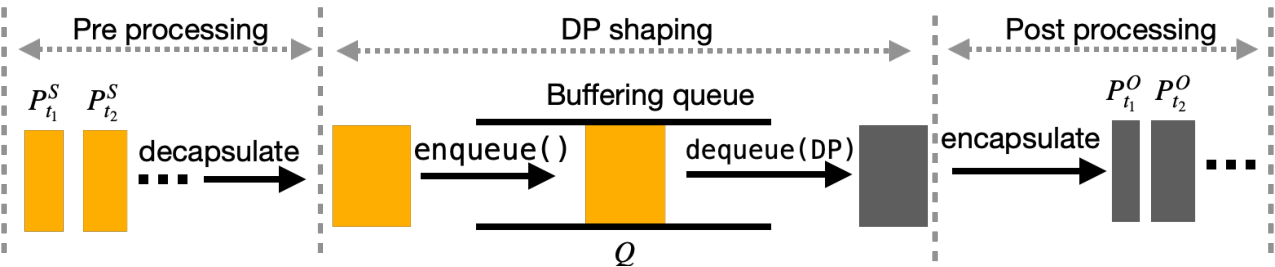
\includegraphics[width=\columnwidth]{figures/DPshaping_concept_vertical.pdf}
  %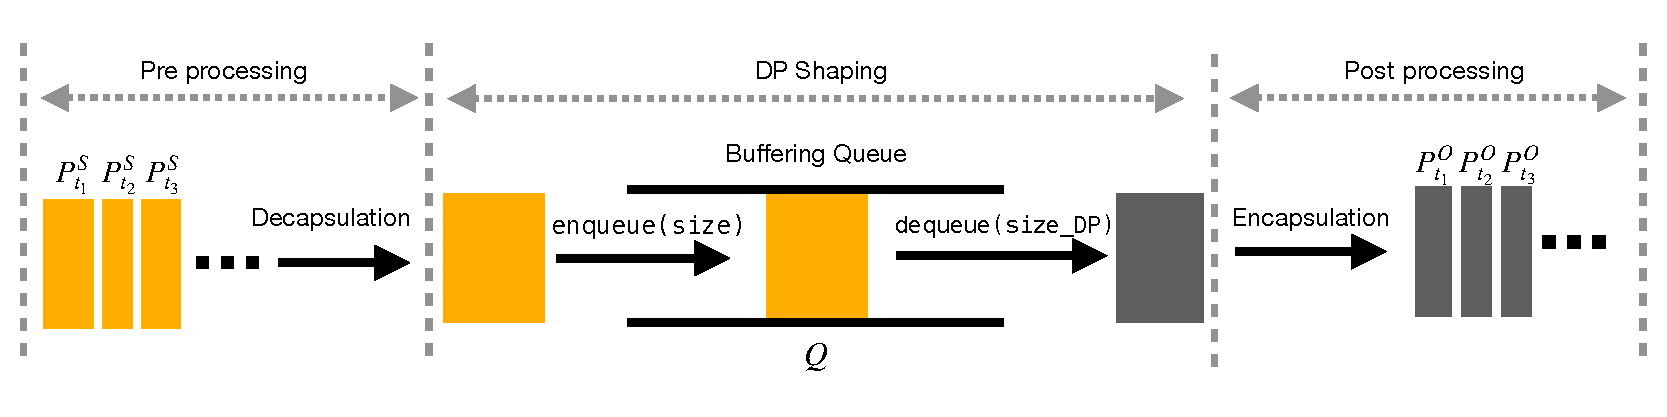
\includegraphics[width=\columnwidth]{figures/DPshaping_concept_horizontal.pdf}
  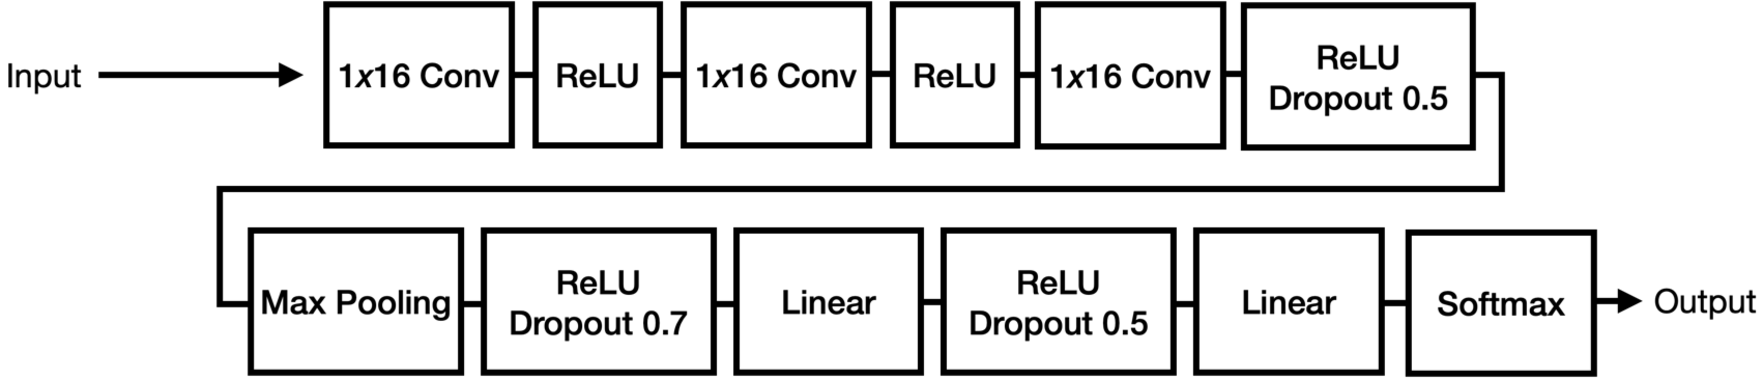
\includegraphics[width=\columnwidth]{figures/BandB_arch.pdf}
  \caption{Beauty and The Burst CNN model architecture.}
  \label{fig:bandb-arch}
\end{figure}

\subsection{Website Fingerprinting}
Website fingerprinting is similar to video identification.
In website fingerprinting attacks, the attacker goal is to map the victim's packet sequence to the website that the victim visits. 
Deep Neural Networks (DNNs) are shown to be effective in website fingerprinting attacks~\cite{sirinam2018df}.
However, due to the differences in characteristics of website traffic compared to video streaming applications, website fingerprinting attacks use different features and model architectures. 
A notable contrast distinguishing video from web traffic traces is the comparatively shorter duration of web traces compared to the more extended durations typical of video traces.
Sirinam~\etalc{sirinam2018df} show that a small CNN with one convolutional layer is able to map users' traffic to their content with 98\% accuracy.
They further show that their model is able to achieve 90\% accuracy in the presence of WTF-PAD~\cite{juarez2016wtfpad} defense mechanism (see \Cref{subsubsec:wtf-pad}), and it achieves 49.7\% accuracy when Walke-Talkie~\cite{wang2017walkie} is deployed (see \Cref{subsubsec:walkie-talkie}).
This highlights the ineffectiveness of ad-hoc shaping mechanisms in face of emerging attacks.

